% 24.04.2015

\section{Eigenwerte und Eigenvektoren}

Die Rolle der Eigenwerte und Eigenvektoren in der linearen Algebra und deren Anwendungen innerhalb und außerhalb der Mathematik ist absolut zentral. Egal ob man ein lineares Gleichungssystem auf Stabilität analysiert, ein System von linearen Differnetialgleichungen löst, Eigenschaften einer Markov-Kette untersucht, oder ein iteratives Verfahren benutzt, um ein nichtlineares Optimierungsproblem zu lösen, braucht man Eigenwerte und Eigenvektoren. Eigenwerte und Eigenvektoren geben einem in der Regel die wichtigste Information über die zugrundeliegende lineare Abbildung eines Veketorraums bzw. über die zugrundeliegende Matrix. 

\subsection{Grundlagen}

In diesem Abschnitt geben wir die Grunddefinitionen Eigenwert und Eigenvektor und beweisen die ersten, nützlichen Resultate darüber.

\subsubsection{Beispiele und Motivation}\label{motiv:eigenwerte}

Das Ziel, dass man bei der Berechnung von Eigenwerten und Eigenvektoren verfolgt ist, eine gegebene lineare Abbildung eines endlichdimensionalen Vektorraums als \textquote{Zusammensetzung} von linearen Abbildungen auf Vektorräumen einer kleineren Dimension darstellen. 
Das geht nicht immer, aber es gibt Situationen, in denen man sogar die gegebene lineare Abbildung als Zusammensetzung der linearen Abbildungen eindimensionaler Vektorräume darstellen kann (das ist der günstigste Fall). Etwas formaler beschrieben, ist man auf der Suche nach einer Basis $\mathcal{B}$ für eine gegebene lineare Abbildung $F: V \to V$ eines endlichdimensionalen Vektorraums $V$, in der die Matrix $F_{\mathcal{B}}$ der Abbildung eine möglichst einfache Struktur hat. Am glücklichsten ist man, wenn man eine Basis findet, in der die Matrix der Abbildung diagonal ist. 

Beispiele:
\begin{enumerate}
	\item
		Die Spiegelung $ x = (x_1,x_2) \mapsto (x_1, -x_2) $ auf $ \K^2 $ bzgl. der $x_1$-Achse zerfällt in die folgenden zwei lineare Abbildungen eindimensionaler Unterräume von $\K^2$: 
		
		\begin{center}
		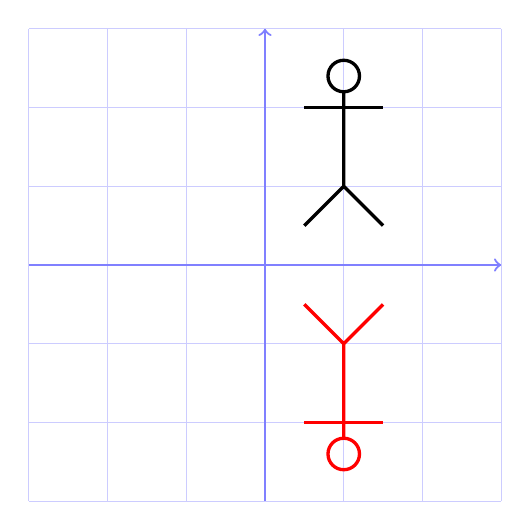
\begin{tikzpicture}
			\draw[blue!20!white] (-3,-3) grid (3,3);
			\draw[blue!50!white,->,thick] (0,-3) -- (0,3);
			\draw[blue!50!white,->,thick] (-3,0) -- (3,0);
			\draw[very thick] (0.5,0.5) -- (1,1) -- (1,2.2) -- (1,1) -- (1.5,0.5);
			\draw[very thick] (0.5,2) -- (1.5,2);
			\draw[very thick] (1,2.4) circle (0.2);
			\draw[red, very thick] (0.5,-0.5) -- (1,-1) -- (1,-2.2) -- (1,-1) -- (1.5,-0.5);
			\draw[red, very thick] (0.5,-2) -- (1.5,-2);
			\draw[red, very thick] (1,-2.4) circle (0.2);
		\end{tikzpicture}
		\end{center} 
	
		\begin{enumerate}
			\item die Identische Abbildung $ x \mapsto x $ auf der Geraden $ \lin(e_1) =\K \times \{ 0 \} $ und
			\item die Spiegelung $ x \mapsto -x $ auf der Geraden $ \lin(e_2) = \{ 0 \} \times \K $.
		\end{enumerate}
		
		Diese Abbildung des Raums $\K^2$ ist also eine \textquote{Zusammensetzung} von zwei linearen Abbildungen von eindimensionalen Räumen. Mit anderen Worten: die Abbildung schickt $e_1$ auf $e_1$ und $e_2$ auf $-e_2$. Die Abbildung ist durch diese Vorgabe eindeutig beschrieben, da eine lineare Abbildung durch die Angabe ihrer Wirkung auf einer Basis eindeutig festgelegt ist. Da $e_1$ auf $e_1$ geschickt wird, fällt man bei der Anwendung der Abbildung auf den Vektoren aus der Geraden $\lin(e_1)$ nicht aus dieser Geraden aus. Ebenso fällt man nicht aus der Geraden $\lin(e_2)$ aus. 
	\item
		Ein weiteres ähnliches Beispiel ist die Projektion $ x = (x_1,x_2) \mapsto (x_1,0) $ auf die $x_1$-Achse in $ \K^2 $. Diese zerfällt in 
		\begin{enumerate}
			\item Die identische Abbildung $ x \mapsto x $ auf der $x_1$-Achse$ \lin(e_1)= \K \times \{ 0 \} $ und
			\item Die Nullabbildung $ x \mapsto 0 $ auf der $x_2$-Achse $\lin(e_2)= \{ 0 \} \times \K $.
		\end{enumerate}
			\begin{center}
		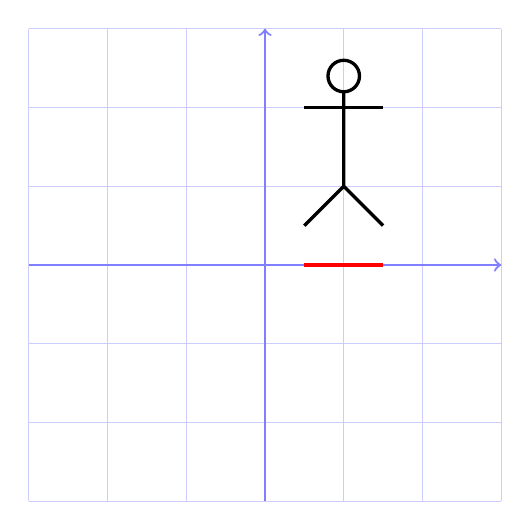
\begin{tikzpicture}
		\draw[blue!20!white] (-3,-3) grid (3,3);
		\draw[blue!50!white,->,thick] (0,-3) -- (0,3);
		\draw[blue!50!white,->,thick] (-3,0) -- (3,0);
		\draw[very thick] (0.5,0.5) -- (1,1) -- (1,2.2) -- (1,1) -- (1.5,0.5);
		\draw[very thick] (0.5,2) -- (1.5,2);
		\draw[very thick] (1,2.4) circle (0.2);
		\draw[red, very thick] (0.5,0) -- ( 1.5,0);
		\end{tikzpicture}
	\end{center} 
	
	\item Bei den vorigen beiden Abbildungen war die Zerlegung direkt erkennbar, weil die zugrundeliegenden Untervektorräume von $\K^2$ Koordinatenachsen waren. Hier noch ein Beispiel, in dem man ebenfalls eine Zerlegung findet, aber nicht bzgl. der Koordinaten Achsen. 
		Wir betrachten die Abbildung $ x = (x_1,x_2) \mapsto (x_2,x_1) $ auf $ \K^2 $. Diese Abbildung ist wie auch das erste Beispiel ebenfalls eine Spiegelung.
		\begin{enumerate}
			\item $ x \mapsto x $ auf der Geraden $ \{ (x_1,x_2) \in \K^2 : x_1 = x_2 \} $ und
			\item $ x \mapsto -x $ auf der Geraden $ \{ (x_1,x_2) \in \K^2 : x_1 = - x_2 \} $.
		\end{enumerate}
			\begin{center}
	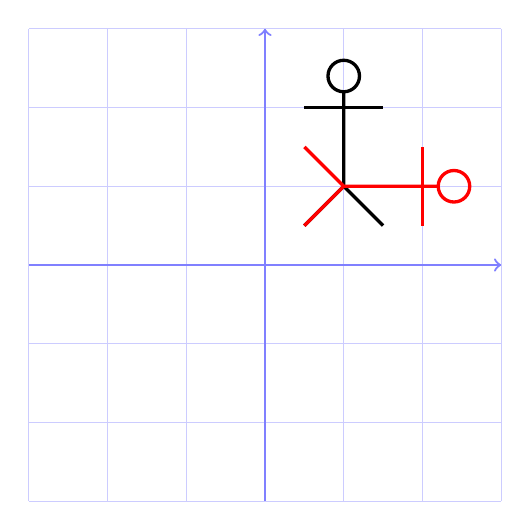
\begin{tikzpicture}
	\draw[blue!20!white] (-3,-3) grid (3,3);
	\draw[blue!50!white,->,thick] (0,-3) -- (0,3);
	\draw[blue!50!white,->,thick] (-3,0) -- (3,0);
	\draw[very thick] (0.5,0.5) -- (1,1) -- (1,2.2) -- (1,1) -- (1.5,0.5);
	\draw[very thick] (0.5,2) -- (1.5,2);
	\draw[very thick] (1,2.4) circle (0.2);
	\draw[red,very thick] (0.5,0.5) -- (1,1) -- (2.2,1) -- (1,1) -- (0.5,1.5);
	\draw[red,very thick] (2,0.5) -- (2,1.5);
	\draw[red,very thick] (2.4,1) circle (0.2);
	\end{tikzpicture}
	\end{center}

	\item
		Nun betrachten wir ein Links-Shift der Koordinaten $ (x_1,x_2) \mapsto (x_2,0) $ auf $ \K^2 $.
		Die Vektoren in der $x_1$-Achse bleiben nach der Anwendung der Abbildung in der $x_1$-Achse, denn sie werden auf $0$ abgebildet: 
		$ x \mapsto 0 $ auf $ \lin(e_1) = \K \times \{ 0 \} $. 
		Man findet aber keinen einen anderen eindimeinsionalen Untervektorraum von $\K^2$ mit der Eigenschaft, dass die Vektoren dieses Untervektorraums nach der Anwendung der Abbildung im fixierten Untervektorraum bleiben. 
		Diese Abbildung lässt sich also nicht als Zusammensetzung von Abbildungen eindimensionaler Untervektorräume darstellen. 
\end{enumerate}

\subsubsection{Definition von Eigenwerten und Eigenvektoren}

Nun haben wir genug Motivation für die Begriffe Eigenwert und Eigenvektor. 
Sei $ V $ Vektorraum über $ \K $ und sei $ F : V \to V $ lineare Abbildung. Ein Paar $(\lambda,v)$ aus einem Skalar $\lambda \in \K$  und einem Nichtnullvektor $ v \in V \setminus \{ 0 \} $ mit der Eigenschaft
\begin{equation}
	F(v) = \lambda v
\end{equation}
heißt \emph{Eigenpaar} von $F$. Dabei heißt $\lambda$ \emph{Eigenwert} von $F$ und $v$ \emph{Eigenvektor} zum Eigenwert $\lambda$ von $F$. 

Sie können nun Beispiele aus \ref{motiv:eigenwerte} nochmals betrachten und alle Eigenpaare der in \ref{motiv:eigenwerte} angegebenen linearen Abbildungen finden. Wenn wir in einem Eigenpaar $(\lambda,v)$ den Eigenvektor $v$ mit einem Nichtnullwert $\alpha \in \K \setminus \{0\}$ multiplizieren, so erhalten wir ein Eigenpaar $(\lambda, \alpha v)$, das sich im Wesentlichen von dem ursprünglichen Eigenpaar $(\lambda,v)$ nicht unterscheidet. Mit anderen Worten ist nur die Richtung eines Eigenvektors wichtig. Die genaue Skalierung des Eigenvektors des spielt keine Rolle. 

Analog werden diese Begriffe Eigenpaar, Eigenwert und Eigenvektor für eine quadratische Matrix eingeführt. Die Eigenwerte, Eigenvektoren und Eigenpaare von $ A \in \K^{n \times n} $ sind jene der zugehörigen Abbildung $ x \mapsto Ax $, oder ausformuliert: $(\lambda,v)$ mit $\lambda \in \K$ und $v \in \K^n \setminus \{0\}$ ist \emph{Eigenpaar} von $A$, wenn die Bedingung $A v = \lambda v$ erfüllt ist. 

\begin{bem}
Wie bereits in Teil~1 des Kurses erwähnt ermöglichen Matrizen eine konkrete Beschreibung der linearen Abbildung im ``konkreten Raum'' $\K^n$. Da man im Raum $\K^n$ die Standardbasis $e_1,\ldots,e_n$ hat, ist es naheliegend die Wirkung einer Abbildung des Raums $\K^n$ genau in dieser Basis festzuliegen. Genau dass macht die Matrix $A$ der Abbildung $x \mapsto A x$. Die Standardbasis ist aber nicht notwendigerweise eine Basis, in der man die zugrundeliegende Abbildung am besten versteht. Das ist einer der Gründe, warum der abstrakte Zugang zur linearen Algebra durch allgemeine Vektorräume $V$ günstig ist: man legt keine feste Basis fest. Des Weiteren muss man noch bedenken, dass nicht jeder Vektorraum eine Standardbasis hat. Tatsächlich hat zum Beispiel die Ebene $ E:= \{ (x,y,z) \, :\, x + 2 y - 3 z = 0 \} \subseteq \R^3$ keine Standardbasis, man kann aber stets eine Basis $b_1, b_2$ wählen und danach diese Ebene als $\R^2$ behandeln. Man kann z.B. eine $90$-Grad Drehung $ F: E \to E$ in der Ebene $E$ betrachten und analysieren. Wenn wir die lineare Algebra ausschließlich konkret auf der Basis von Vektoren aus $\K^n$ und Matrizen entwickelt hätten, hätten wir keine Sprache zur Verfügung zur Einführung und der Behandlung der Drehung $F$ wie oben. 
\end{bem}

\begin{bem}
	Es ist klar, dass der Begriff vom Kern
	$\ker(F)$ einer linearen Abbildung $F : V \to V$ mit Eigenvektoren zusammenhängt. Nichtnullvektoren aus dem Kern sind genau die Eigenwerte von $F$ zum Eigenwert $0$. 
\end{bem}

\begin{bem}
Ein Eigenvektor $v$ zum Eigenwert $1$ hat die Eigenschaft $F(v) = v$, das heißt, $v$ ist ein sogenannter Fixpunkt der Abbildung $v$. Solche Fixpunkte sind oft von einem besonderen Interesse. Der Vektor der Google-Pageranks der Internetseiten ist ein Fixpunkt einer linearen Abbildung, die durch die Vernetzung der Internetzung der Internetseiten bestimmt ist.
\end{bem}

\begin{bem}
Die Aufgaben $A x = b$ (Lösung von linearen Gleichungssystemen) und $A v = \lambda v$ (Eigenwertaufgabe) sind die zwei Grund-Rechenaufgaben der linearen Algebra. In der Numerik werden Sie verschiedene Methoden zur Lösung dieser zwei Aufgaben lernen. Die beiden Aufgaben sind nämlich der Hauptgegenstand der Numerischen Linearen Algebra. 

Hierbei wählt man $\C$ als den zugrundeliegenden Körper und führt die Berechnungen in der Praxis annähernd mit Hilfe der sogenannten Gleitkommazahlen.  Die Aufgabe $A v = \lambda v$ kann etwas konkreter in verschiedenen Varianten gestellt werden. In der numerischen Mathematik interessiert man sich oft für den Eigenwert $\lambda$ mit dem höchsten Betrag und einen zugehörigen Eigenvektor. Alle Rechenaufgaben aus der linearen Algebra, die wir bis jetzt betrachtet haben, konnten wir durch das Gauß-Verfahren (bzw. eine Variation davon) lösen. Die Eigenwertaufgabe ist aber die Aufgabe, bei der das Gauß-Verfahren \textbf{nicht} direkt hilft (man braucht weitere Ideen). Die Aufgabe ist eigentlich nicht linear, denn $\lambda$ ist unbekannt, $v$ ist ebenfalls unbekannt und die Aufgabe $A v = \lambda v$ enthält das \textbf{Produkt} dieser unbekannten Objekte. Sobald man das Unbekannte $v$ oder $\lambda$ bestimmt hat, ist man im Wesentlichen durch. Kennt man das $v$, so ermittelt man $\lambda$ als Streckungsfaktor der parallelen Vektoren $A v$ und $v$. Hat man $\lambda$ ermittelt, so reduziert sich die Bestimmung eines zugehörigen Eigenvektors zur Lösung des LGS $A v= \lambda v$ für einen unbekannten Vektor $v$.
\end{bem}

%\begin{bem}
%	Die Schwingung einer Feder ohne Dämpfung wird durch die lineare Differentialgleichung $m x''(t) + k x(t) = 0$ ($m$ Masse, $k$ die Federkonstante) die Startbedingungen beschrieben. Zu dieser Gleichung kann man die lineare Abbildung betrachten, welche der Funktion $x(t)$ die Funktion $m x''(t) + k x(t)$ zuordnet. Die Eigenwerte dieser lineare Abbildung heißen die Eigenfrequenzen. Bei $m=k=1$ hat man zum Bespiele die Lineare Abbildung $ x(t) \mapsto x''(t) + x(t)$. 
%\end{bem}

\subsubsection{Diagonalisierbarkeit von linearen Abbildungen}

Hier und im Folgenden sei $n \in \N$.
Sei $ V $ ein $ n $-dimensionaler Vektorraum über $ \K $. Eine Abbildung $ F \in \Lin(V) $ heißt diagonalisierbar, wenn eine Basis $ \mathcal{B} $ von $ V $ existiert, für welche die Matrix $ F_\mathcal{B} $ diagonal ist. Die Diagonalisierbaren Abbildungen sind die einfachsten Abbildungen in der Theorie der Eigenwerte und Eigenvektoren. 

Die nachfolgende Proposition formuliert Diagonalisierbarkeit in der Sprache der Eigenwerte und Eigenvektoren. 

\begin{propn}
	Sei $ V $ ein $ n $-dimensionaler Vektorraum und sei $ F \in \Lin(V) $. Dann sind die folgenden Bedingungen äquivalent:
	\begin{enumerate}
		\item
			$ F $ ist diagonalisierbar.
		\item
			$ V $ besitzt eine Basis aus Eigenvektoren von $ F $.
	\end{enumerate}
\end{propn}
\begin{proof}
	Um diese Proposition herzuleiten, reicht es aus, die Definition von $F_\mathcal{B}$ auszuschreiben. Die Matrix $F_\mathcal{B}$ der Abbildung $F$ bzgl. der Basis $\mathcal{B} = (b_1,\ldots,b_n)$ entsteht folgendermaßen: man wenden $F$ zu den Basisvektoren $b_1,\ldots,b_n$ und schreibt das Ergebnis jedes mal wieder in der Basis $b_1,\ldots,b_n$ auf. Die $i$-te Spalte enthält die Darstellung von $F(b_i)$ in der Basis $b_1,\ldots,b_n$. Die Eigenschaft, dass $F_\mathcal{B}$ diagonal mit Diagonalelementen $\lambda_1,\ldots,\lambda_n$ ist, bedeutet als, dass $f(b_i) = \lambda_i b_i$ erfüllst. Das heißt, $\mathcal{B}$ ist Basis aus Eigenvektoren von $F$, und die jeweiligen Diagonalelemente sind die entsprechenden Eigenwerte.
\end{proof}

\begin{bsp}[aus 6.1.1]
	Sei $ F(x_1,x_2) = (x_2,x_1) $. Dann ist $ b_1 = (1,1) $ Eigenvektor zum Eigenwert 1, $ b_2 = (-1,1) $ Eigenvektor zum Eigenwert -1 und $ \mathcal{B} = (b_1, b_2) $ eine Basis von $ \Q^2 $. D.h.
	\begin{equation*}
		F_\mathcal{B} = \begin{pmatrix}
			1 & 0 \\
			0 & -1
		\end{pmatrix}
	\end{equation*}
\end{bsp}
\begin{bsp}[aus 6.1.1]
	Sei $ F(x_1,x_2) = (x_2,0) $. Dies ist ein Beispiel einer ``problematischen'' Abbildung, welche man nicht diagonalisieren kann. Zeigen wir das durch ein Widerspruchsargument. Angenommen, $F$ hätte eine Basis $b_1,b_2$ aus Eigenvektoren mit den jeweiligen Eigenwerten $\lambda_1$ und $\lambda_2$. Die zweifache Anwendung von $F$ zu einem beliebigen Vektor aus $\K^2$ ergibt null ( $(x_1,x_2) \mapsto (x_2,0) \mapsto (0,0)$ ). Das heißt $F^2(x) =0$ für alle $x$. Wir haben aber $F(b_i) = \lambda_i b_i$ und somit $F^2(b_i) = F(\lambda_i b_i) = \lambda_i F(b_i) = \lambda_i^2 b_i$. Also ist $\lambda_i^2 b_i = 0$. Da $b_i$ kein Nullvektor ist, folgt $\lambda_i^2 = 0$. Daraus folgt $\lambda_i =0$. Wir haben $\lambda_1 = \lambda_2 = 0$. Unser Abbildung schickt somit den Basisvektor $b_i$ auf den Vektor $0 b_i =0$. Somit ist $F$ eine Nullabbildung, das widerspricht aber zu $F(e_2) = e_1 \ne 0$.
\end{bsp}

Durch die vorigen Beispiele sehen wir, dass man unproblematische (diagonalisierbare) sowie problematische (nichtdiagonalisierbare) Abbildungen hat. Wir sind an der Theorie interessiert, die uns helfen würde, die beiden Fälle auseinanderzuhalten. Im Rest des Kapitels werden Werkzeuge dazu entwickelt. 

Im Rest dieses Abschnitts besprechen wir noch  kurz die Diagonalisierbarkeit von quadratischen Matrizen. Eine Matrix $ A \in \K^{n \times n} $ heißt diagonalisierbar, wenn die lineare Abbildung $ x \mapsto Ax $ auf $ \K^n $ diagonalisierbar ist, 
mit anderen Worten: $ \K^n $ besitzt eine Basis $ b_1, \ldots, b_n $ mit $ Ab_i = \lambda_ib_i \enspace\forall i \in \is{1}{n} $, wobei $ \lambda_1, \ldots, \lambda_n \in \K $. Aus dieser Definition wird deutlich, dass die Eigenschaft von der Wahl des Körpers abhängig ist. Eine Matrix $A \in \R^{n \times n}$ ist auch eine Matrix aus $\C^{n \times n}$. Es gibt Fälle, in den $A$ bzgl. $\R$ nicht diagonalisierbar ist, aber bzgl. des größeren Körpers $\C$ diagonalisierbar. Mehr dazu später. 


\begin{propn}
	Sei $ A \in \K^{n \times n} $. Die Matrix $ A $ ist genau dann diagonalisierbar (bzgl. $\K$), wenn eine invertierbare Matrix $ B \in \K^{n \times n} $ existiert, sodass $ B^{-1}AB $ diagonal ist.
\end{propn}
\begin{proof}
	Wie der vorige Beweis brauchen wir auch hier, lediglich die Diagonalisierbarkeit in eine andere Sprache zu übersetzen, und zwar in die Sprache der Matrizen. 
	Sei $ A $ diagonalisierbar, d.h. es existiert eine Basis $ b_1, \ldots, b_n $ von $ \K^n $ mit $ Ab_i = \lambda_ib_i \enspace\forall i \in \is{1}{n} $, wobei $ \lambda_1, \ldots, \lambda_n \in \K $. Sei $ B = (b_1, \ldots, b_n) $. Dann ist
	\begin{equation*}
		A \begin{pmatrix}
			| && | \\
			b_1 & \cdots & b_n \\
			| && |
		\end{pmatrix} = \begin{pmatrix}
			| && | \\
			\lambda_1b_1 & \cdots & \lambda_nb_n \\
			| && |
		\end{pmatrix} = \begin{pmatrix}
			| && | \\
			b_1 & \cdots & b_n \\
			| && |
		\end{pmatrix} \begin{pmatrix}
			\lambda_1 && \\
			& \ddots & \\
			&& \lambda_n
		\end{pmatrix}
	\end{equation*}
	$ B $ ist invertierbar, weil die Spalten von $ B $ eine Basis bilden (vgl. LA I). Wir multiplizieren die vorige Gleichung mit $ B^{-1} $ von links und erhalten
	\begin{equation}
		B^{-1}AB = \begin{pmatrix}
			\lambda_1 && \\
			& \ddots & \\
			&& \lambda_n
		\end{pmatrix}
		\label{eq:6_1_3}
	\end{equation}
	Umgekehrt: sei $ B \in \K^{n \times n} $ eine invertierbare Matrix, für welche $ B^{-1}AB $ diagonal ist, d.h. \eqref{eq:6_1_3} gilt mit $ \lambda_1, \ldots, \lambda_n \in \K $. Es folgt: $ b_1, \ldots, b_n $ ist eine Basis von $ \K^n $ mit $ Ab_i = \lambda_ib_i \enspace\forall i \in \is{1}{n} $.
\end{proof}

\noindent Motiviert durch die vorige Proposition führen wir den Begriff der Ähnlichkeit von Matrizen ein. Matrix $ A \in \K^{n \times n} $ und $ \widetilde{A} \in \K^{n \times n} $ heißen \emph{ähnlich}, wenn eine invertierbare Matrix $ B \in \K^{n \times n} $ existiert mit $ B^{-1}AB = \widetilde{A} $.
Die Ähnlichkeit von Matrizen ist eine Äquivalenzrelation (Zeigen Sie das). 

\begin{bsp}
	$ \widetilde{A} = \begin{pmatrix}
		1 & 0 \\
		0 & -1
	\end{pmatrix}, A = \begin{pmatrix}
		0 & 1 \\
		1 & 0
	\end{pmatrix} \in \Q^2 $. Seien $ b_1 = \begin{pmatrix}
		1 \\ 1
	\end{pmatrix}, b_2 = \begin{pmatrix}
		1 \\ -1
	\end{pmatrix} $. Dann ist $ Ab_1 = b_1 $, $ Ab_2 = -b_2 $. D.h. für $ B = (b_1, b_2) $ ist $ AB = B\widetilde{A} \Leftrightarrow B^{-1}AB = \widetilde{A} $. Die Matrix $\widetilde{A}$ beschreibt eine Spiegelung an der $x_2$-Achse, die Matrix $A$ eine Spiegelung an der Achse $x_1=x_2$. Die Matrizen machen also tatsächlich was Ähnliches. 
\end{bsp}

In Bezug auf die Theorie der Eigenwerte und Eigenvektoren unterscheiden sich zwei verschiedene ähnliche Matrizen voneinander nicht (d.h., sie haben komplett die gleichen Eigenschaften in dieser Theorie).

\subsubsection{Diagonalisierbarkeit: eine hinreichende Bedingung}
\label{sec:6_1_4}

Wir diskutieren hier eine Bedingung, die in vielen Situationen hilft, Diagonalisierbarkeit zu erkennen. Bei der Diagonalisierung geht es um die Suche nach einer Basis, in der die Abbildung diagonal ist. Die Vektoren der Basis sollen Eigenvektoren sein. Wir sind als auf der Suche nach linear unabhängigen Eigenvektoren. Das folgende Lemma zeigt, dass wir im Fall von verschiedenen Eigenwerten, die lineare Unabhängigkeit geschenkt bekommen. 

\begin{lm}
	Sei $F: V \to V$ lineare Abbildung über einem Vektorraum $V$ und
	seien $ (\lambda_1,v_1), \ldots, (\lambda_m,v_m) $ Eigenpaare von $ F $ mit der Eigenschaft, dass $ \lambda_1, \ldots, \lambda_m $ \emph{paarweise verschieden} sind. Dann sind $ v_1, \ldots, v_m $ linear unabhängig.
\end{lm}
\begin{proof}
	Induktion über $ m \in \N $. Für $ m = 1 $ ist die Behauptung trivial. Angenommen, die Behauptung gilt für $ m-1 $ Eigenpaare mit $m \ge 2$. Wir betrachten nun $m$ Eigenpaare mit $m$ verschiedenen Eigenwerten. Seien $ \alpha_1, \ldots, \alpha_m \in \K $ beliebige Skalare mit
	\begin{equation}
		\alpha_1v_1 + \ldots + \alpha_mv_m = 0
		\label{eq:6_1_4}
	\end{equation}
	Wir multiplizieren \eqref{eq:6_1_4} mit $ \lambda_m $ und erhalten:
	\begin{equation*}
		\lambda_m\alpha_1v_1 + \ldots + \lambda_m\alpha_{m-1}v_{m-1} + \lambda_m\alpha_mv_m = 0
	\end{equation*}
	Die Anwendung von $ F $ zu \eqref{eq:6_1_4} ergibt:
	\begin{equation*}
		\lambda_1\alpha_1v_1 + \ldots + \lambda_m\alpha_mv_m = 0
	\end{equation*}
	In der Differenz der vorigen zwei Gleichungen verschwindet der Term mi $v_m$:
	\begin{equation*}
		(\lambda_1 - \lambda_m)\alpha_1v_1 + \ldots + (\lambda_{m-1} - \lambda_m)\alpha_{m-1}v_{m-1} = 0
	\end{equation*}
	% 04.05.2015
	Nach Induktionsvoraussetzung sind $ v_1, \ldots, v_{m-1} $ linear unabhängig. Also folgt aus der vorigen Gleichung, dass alle Koeffizienten der linearen Kombination auf der linken Seite gleich $0$ sind:
	\begin{equation*}
		(\lambda_1 - \lambda_m)\alpha_1 = \ldots = (\lambda_{m-1} - \lambda_m)\alpha_{m-1} = 0
	\end{equation*}
	Da die Eigenwerte paarweise verschieden sind, ist $ \lambda_i - \lambda_m \neq 0 $ für alle $ i \in \is{1}{m-1} $,l erhält man
	\begin{equation*}
		\alpha_1 = \ldots = \alpha_{m-1} = 0
	\end{equation*}
	Das Einsetzen in \eqref{eq:6_1_4} ergibt $ \alpha_m v_m = 0 $. Mit $ v_m \neq 0 $ folgt $ \alpha_m = 0 $. Wir haben aus \eqref{eq:6_1_4} $\alpha_1 = \cdots = \alpha_m =0$ erhalten. D.h., $ v_1, \ldots, v_m $ sind linear unabhängig.
\end{proof}

\begin{thm} 
	Sei $ F : V \to V$ lineare Abbildung eines $n$-dimensionalen Vektorraums $V$, welche $n$ paarweise verschiedene Eigenwerte $ \lambda_1, \ldots, \lambda_n \in \K$ besitzt. Dann ist $ F $ diagonalisierbar.
\end{thm}
\begin{proof}
	Das vorige Lemma ergibt, dass die Eigenvektoren $b_1,\ldots,b_n$ zu den Eigenwerten $\lambda_1,\ldots,\lambda_n$ eine Basis von $V$ bilden. Die Matrix von $F$ bzgl. dieser Basis ist diagonal. 
\end{proof}

Wann ist eine hinreichende Bedingung für eine gewünschte Eigenschaft nützlich? In der Regel wünscht man sich eine möglichst allgemeine hinreichende Bedingung, also eine Bedingung, die nicht zu restriktiv ist. Aus dieser Perspektive ist die oben präsentierte hinreichende Bedingung der Diagonalisierbarkeit zumindest bzgl. des Körpers der komplexen Zahlen \textbf{sehr} nützlich.  Denn diese Bedingung ist bzgl. $\C$ generisch erfüllt: wenn Sie etwa eine Matrix $A$ aus $\C^{n \times n}$ generieren, in dem Sie die $n^2$ Komponenten von $A$ aus einem Bereich, etwa aus dem Segment $[-1,1]$ gleichmäßig und unabhängig ziehen, dann kriegen Sie mit Wahrscheinlichkeit $1$ eine Matrix mit $n$ paarweise verschiedenen Eigenwerte in $\C$. ``Generisch erfüllt'' ist aber nicht nicht das selbe wie (bedingungslos) ``erfüllt''. Wenn sie zwei unabhängige gleichmäßig verteilte Werte $x,y$ aus $[0,1]$ ziehen, dann ist die Eigenschaft $x \ne y$ generisch erfüllt (es ist also unwahrscheinlich, dass $x=y$ gilt). Es gibt zwar Werte $x,y \in [0,1]$ mit $x =y$, diese Werte bilden eine eindimensionale Ausnahme im Quadrat aller Paare $(x,y) \in [0,1]^2$. 


\subsubsection{Eigenraum}

Alle Eigenwerte zu einem festen Eigenwert plus der Nullvektor bilden einen Untervektorraum, den sogenannten Eigenraum. Sei $F: V \to V$ lineare Abbildung eines Vektorraums $V$ und sei $\lambda \in \K$. Dann heißt
\begin{equation}
	\Eig(F,\lambda) := \{ v \in V : F(v) = \lambda v \}
\end{equation}
der \emph{Eigenraum} von $ F $ bzgl. $ \lambda $. Wir setzen in dieser Definition nicht voraus, dass $\lambda$ Eigenwert von $F$ ist. Wenn $\lambda$ kein Eigenwert ist, dann enthält $\Eig(F,\lambda)$ nichts außer dem Nullvektor. Fassen wir die Grundeigenschaften der Eigenräume zusammen: 

\begin{propn}
	Für eine lineare Abbildung $F : V \to V$ eines Vektorraums $V$ und ein $\lambda \in V$ gilt: 
	\begin{enumerate}
		\item
			$ \Eig(F,\lambda) $ ist Untervektorraum von $ V $.
		\item
			$ \lambda $ ist genau dann Eigenwert von $ F $, wenn $ \Eig(F,\lambda) \neq \{ 0 \} $ gilt.
		\item
			Wenn $ \lambda $ Eigenwert von $ F $ ist, dann gilt für $ v \in V $:
			
			$ v $ ist Eigenvektor von $ F $ zu $ \lambda \Longleftrightarrow v \in \Eig(F,\lambda) \setminus \{ 0 \} $
		\item
			$ \Eig(F,\lambda) = \ker(\lambda \id_V - F) $
		\item
			Wenn $ \lambda_1, \lambda_2 \in \K $ verschieden sind, dann gilt $ \Eig(F,\lambda_1) \cap \Eig(F,\lambda_2) = \{ 0 \} $.
	\end{enumerate}
\end{propn}
\begin{proof}
	(i) - (iv) klar, (v) folgt aus dem Lemma in \ref{sec:6_1_4} im Fall $ m = 2 $.
\end{proof}

Durch die Einführung von $\Eig(F,\lambda)$ und die Bemerkung $\Eig(F,\lambda) = \ker(\lambda \id - F)$ schaffen wir mehr Ordnung in unserer Diskussion der Eigenwerte und Eigenvektoren. Jedem Eigenwert $\lambda$ wird nun ein Vektorraum zugeordnet $\Eig(F,\lambda)$, in dem alle Eigenvektoren zu $\lambda$ enthalten sind und der als Kern der Abbildung $\lambda \id - F$ beschrieben werden kann. Wegen (v) gibt es paarweise keine ``Überlappungen'' der Räume $\Eig(F,\lambda)$ (bis auf den Nullvektor, der in jedem Vektorraum enthalten ist). 

\clearpage
\subsection{Das charakteristische Polynom}

Betrachten wir die Version der Eigenwertaufgabe, in der man \text{alle} Eigenwerte bestimmen möchte. Es stellt sich heraus, dass die Eigenwerte die Nullstellen eines besonderen Polynoms sind, das man einer Matrix bzw. einer linearen Abbildung zuordnet. Dieses Polynom wird das charakteristische Polynom genannt. Wenn man das charakteristische Polynome ausrechnen kann, so muss man dann ``nur noch'' die Nullstellen davon berechnen können. 

Am Anfang vom Teil~1 des Kurses haben wir uns kurz mit Polynomen beschäftigt. Hier eine kurze Zusammenfassung vom Wissen über Polynome, das wir in diesem Abschnitt benötigen:

\begin{tcolorbox}[title=Wiederholung]
	Sei $ t $ eine Unbestimmte.
	\begin{itemize}
		\item
			Der Polynomring $ \K[t] $ enthält die Monome $ t^0, t^1, t^2, t^3, \ldots $, wobei $ t^0 $ mit $ 1 $ aus $ \K $ identifiziert wird, und endliche Linearkombinationen dieser Monome mit Koeffizienten aus $ \K $. Das Polynom ist ein formaler Ausdruck (wird also durch die Angabe der Koeffizienten für seine Monome festgelegt).
		\item
			Addition und Multiplikation von Polynomen erfolgt komponentenweise.
		\item
			Die Gleichheit zweier Polynome aus $ \K[t] $ wird durch den Koeffizientenvergleich definiert.
		\item
			Ein Polynom $ f \in \K[t] $ kann an einem $ \lambda \in \K $ ausgewertet werden. Somit definiert jedes $ f \in \K[t] $ die Polynomfunktion $ \lambda \mapsto f(\lambda) $ auf $ \K $.
		\item Polynom ist nicht das gleiche wie Polynomfunktion. Nehmen wir als Beispiel den Körper $\K = \{0,1\}$. Die Polynome $f=t$ und $g=t^2$ in $\K[t]$ bestimmen die selbe Polynomfunktion (die identische Funktion), das sind aber trotzdem verschiedene Polynome. 
	\end{itemize}
\end{tcolorbox}

\subsubsection{Das charakteristische Polynom einer Matrix}

In Kapitel~\ref{Determinanten} über die Determinanten haben aus den Formeln für die Determinanten Formeln für Grundaufgaben der linearen Algebra hergeleitet. Nun sind die Eigenwerte dran, wir erstellen mit der Verwendung der Determinanten eine Gleichung für die Eigenwerte. 

\begin{propn}
	Sei $ A \in \K^{n \times n} $, $ \lambda \in \K $. Dann sind folgende Aussagen äquivalent:
	\begin{enumerate}
		\item
			$ \lambda $ ist Eigenwert von $ A $.
		\item
			$ \det(\lambda I - A) = 0 $.
	\end{enumerate}
\end{propn}
\begin{proof}
	$\lambda$ ist genau dann Eigenwert von $v$, wenn die Gleichung $A v = \lambda v$ eine Nichtnull-Lösung $v$ besitzt. Das bedeutet, dass der Kern der quadratischen Matrix $\lambda I - A$ ungleich Null ist. Das Letztere ist äquivalent zu $\det(\lambda I - A) =0$, wie wir aus dem Kapitel~\ref{Determinanten} über die Determinanten wissen. 
\end{proof}

\noindent Hier und im Folgenden sei $ t $ eine Unbestimmte. Motiviert durch die vorige Proposition möchten wir das charakteristische Polynom $ p_A \in \K[t] $ einer Matrix $ A \in \K^{n \times n} $ durch die Gleichung
\begin{equation} \label{p_A}
	p_A := \det(t I - A)
\end{equation}
einführen. Da wir mathematisch sauber arbeiten wollen, können wir das $p_A$ auf diese Weise  noch nicht bedenkenlos definieren. Schauen wir uns den Ausdruck $\det(t I - A)$ genauer an. $t I - A$ ist die Matrix, deren Komponenten zum Ring $\K[t]$ der Polynome gehören. Etwa im Fall $n=2$:
\[
	 \begin{pmatrix} a_{11} & a_{12} \\ a_{21} & a_{22} \end{pmatrix}  = \begin{pmatrix} t-a_{11} & -a_{12} \\ -a_{21} & t- a_{22} \end{pmatrix} 
\]
Wir betrachten also die Determinante einer Matrix, deren Komponenten zum kommutativen Ring $\K[t]$ gehören. Die Theorie der Determinanten haben wir aber für die Matrizen entwickelt, deren Elemente zu einem Körper gehören. Streng genommen können wir also von dieser Theorie ohne extra Begründung keinen Gebrauch machen. Es ist klar, dass man in die Leibniz-Formel auch Matrizen über einem Ring einsetzen kann, denn in der Leibniz-Formel wird nirgendwo dividiert (es reicht als aus, einen kommutativen Ring zu haben, in dem im Gegensatz zu einem Körper nicht jedes Element invertierbar sein muss). Also könnte man im Prinzip $p_A$ durch die Leibniz-Formel einführen. Aber, das wäre noch kein Ausweg. Denn wir wollen die Theorie der Determinanten benutzen, deren Gültigkeit wir nur im Fall von Matrizen über einem Körper verifiziert. Wir können die Situation ziemlich einfach retten: und zwar werden wir den Ring $\K[t]$ in einen Körper einbetten. 

\subsubsection{Rechtfertigung der Definition vom charakteristischen Polynom}

Es ist lehrreich einen Vergleich mit den ganzen Zahlen zu machen. Von einer Matrix mit ganzzahligen Komponenten $A \in \Z^{n \times n}$ können wir die Determinante berechnen, da der Ring $\Z$ der ganzen Zahlen zum Körper $\Q$ rationaler Zahlen erweitert werden kann. Also gehört $A  \in \Z^{n \times n}$ zu $\Q^{n \times n}$ und somit hat $A$ die Determinante bzgl. des Körpers der rationalen Zahlen. Diese Determinante kann unter anderem durch die Leibniz-Formel berechnet werden, in der nicht dividiert wird. Das zeigt also, das die Determinante einer ganzzahligen Matrix eine ganze Zahl ist.  Obwohl wir die rationalen Zahlen als Hilfstruktur benutzt haben, ist unsere Eingabe $A \in \Z^{n \times n}$ sowie Rückgabe $\det(A)$ ganzzahlig. 


In der Theorie der Ringe und Körper gibt es eine Verallgemeinerung der Konstruktion der rationalen Zahlen aus den ganzen Zahlen. Auf Basis welcher kommutative Ringe $R$ kann man Quotienten $\frac{a}{b}$ mit $a,b \in R$ und $b \ne 0$ einführen? Wenn der Ring $R$ Nullteiler hat, hat man ein Problem. Nehmen wir etwa an, $a$ und $b$ sind zwei Elemente von einem kommutativen Ring $R$ mit eins, die nicht gleich null sind und deren Produkt $a b$ gleich null ist (in $\Z / 6 \Z$ sind es zum Beispiel die Restklassen von $2$ und $3$). Die Quotienten können wir in einem solchen Ring nicht sinnvoll einführen. Im Prinzip könnten wir $\frac{1}{a}$ und $\frac{1}{b}$ betrachten, weil die Nenner ungleich null sind, wenn wir aber die beiden Quotienten multiplizieren  kriegen wir ein Problem: $\frac{1}{a} \cdot \frac{1}{b} = \frac{1}{a b} = \frac{1}{ 0}$. Im Ring der ganzen Zahlen hat man keine Nullteiler, daher lassen sich die Quotienten (also die rationalen Zahlen) korrekt einführen. 

Genau so hat man auch im Polynomring $\K[t]$ keine Nullteiler, und somit hat man auch eine wohldefinierte Weise die Quotienten $\frac{f}{g}$ von Polynomen $f, g \in \K[t]$ mit $g \ne 0$ einzuführen. Die Menge solcher Quotienten, ausgestattet mit den natürlichen Operationen $+$ und $\cdot$, bildet den sogenannten Quotientenkörper $\K(t)$. Es ist keine Überraschung, dass die Addition und Multiplikation folgendermaßen eingeführt werden: 
\begin{align}
\frac{f_1}{g_1} + \frac{f_2}{g_2} &:= \frac{f_1g_2 + f_2g_1}{g_1g_2} \\
\frac{f_1}{g_1} \cdot \frac{f_2}{g_2} &:= \frac{f_1f_2}{g_1g_2}
\end{align}
Des Weiteren lässt sich ein und der selbe Quotient auf mehrere Weisen hinschreiben. Wir müssen also klären, wann zwei Quotienten gleich sind. Hier auch keine Überraschungen: 
\begin{equation}
\frac{f_1}{g_1} = \frac{f_2}{g_2} \quad\Leftrightarrow\quad f_1g_2 = f_2g_1.
\end{equation}
Die Konstruktion des Quotientenkörper kann natürlich auch noch formaler beschrieben werden: ein Quotient ist eine Äquivalenzklasse aus Paaren (Zähler,Nenner) (mit Zähler aus $\K[t]$ und Nenner aus $\K[t] \setminus \{0\}$),  wobei zwei solche Paare $(f_1,g_1)$ und $(f_2, g_2)$ äquivalent sind, wenn $f_1 g_2 = f_2 g_1$ gilt. Sie können sich gerne überlegen, dass die oben angeführten Konstruktionen mathematisch korrekt sind: die eingeführte Relation ist tatsächlich eine Äquivalenzrelation, $+$ und $\cdot$ sind unabhängig davon, durch wie man den Quotienten konkret dargestellt und $\K(t)$ ist tatsächlich ein Körper. 

Der Ring $\K[t]$ wird als Unterstruktur von $\K(t)$ aufgefasst, denn $f \in \K[t]$ wird natürlicherweise mit dem Quotienten $\frac{f}{1}$ identifiziert. 

Nun hat unser Definition des charakteristischen Polynoms $\K[t]$ eine eindeutige Interpretation. Man hat
\[
	p_A := \det ( t I - A).
\]
Die Elemente der Matrix $t I - A$ gehören zum Ring $\K[t]$ und somit auch zum Körper $\K(t)$ der rationalen Funktionen. Somit wissen wir dass $\det(t I - A)$ bzgl. des Körpers $\K(t)$ definiert. Aber aus der Leibniz-Formel (in der nicht dividiert wird) wissen wir, dass $\det( t I - A)$ zum Ring $\K[t]$ gehört.

\begin{bem} \hfill {\normalfont 08.05.2015} \\
	Zur Berechnung von charakteristischen Polynomen können jede Methode aus dem Kapitel~5 benutzen: Leibniz-Formel, Laplace-Entwicklung, Gauß-Verfahren bzgl. des Körpers $ \K(t) $.
\end{bem}

\begin{bsp}
	Hier einige Beispiele der charakteristischen Polynome: 
	\begin{center}
	\begin{tabular}{c|c}
		Matrix & Das charakteristische Polynom \\
		\hline
		$ \begin{pmatrix}
			0 & 0 \\ 0 & 0
		\end{pmatrix} $ & $ \det\begin{pmatrix}
			t & 0 \\ 0 & t
		\end{pmatrix} = t^2 $ \\
		$ \begin{pmatrix}
			0 & 1 \\ 0 & 0
		\end{pmatrix} $ & $ \det\begin{pmatrix}
			t & 1 \\ 0 & t
		\end{pmatrix} = t^2 $ \\
		$ \begin{pmatrix}
			1 & 0 \\ 0 & 0
		\end{pmatrix} $ & $ \det\begin{pmatrix}
			t - 1 & 0 \\ 0 & t
		\end{pmatrix} = (t-1)t = t^2 - t $ \\
		$ \begin{pmatrix}
			1 & 1 \\ 0 & 1
		\end{pmatrix} $ & $ \det\begin{pmatrix}
			t-1 & -1 \\ 0 & t-1
		\end{pmatrix} = (t-1)^2 $ \\
		$ \begin{pmatrix}
			1 & 1 \\ 1 & 1
		\end{pmatrix} $ & $ \det\begin{pmatrix}
			t-1 & -1 \\ -1 & t-1
		\end{pmatrix} = (t-1)^2 - 1 = t(t-2) $ \\
	\end{tabular}
	\end{center}
\end{bsp}

\begin{bem}
	Ist $R$ ein kommutativer Ring mit $1$ und ohne Nullteiler, so ist bildet die Menge der Quotienten $\frac{a}{b}$ mit $a \in R$ und $b \in \R \setminus \{0\}$, zusammen mit $+$ und $\cdot$ (die genauso wie oben eingeführt werden), den sogenannten Quotientenkörper $\operatorname{Quot}(R)$ des Rings $R$. Anhand dieses Körpers kann man die Determinanten der Matrizen aus $R^{n \times n}$ einführen. 
\end{bem}

\subsubsection{Nullstellen, Grad und Koeffizienten des charakteristischen Polynoms}

\begin{propn}
	Sei $ A \in \K^{n \times n} $ mit $ n \in \N $ und $ \lambda \in \K $. Dann sind die folgenden Aussagen äquivalent:
	\begin{enumerate}
		\item
			$ \lambda $ ist Eigenwert von $ A $.
		\item
			$ \lambda $ ist Nullstelle von $ p_A $, d.h. $ p_A(\lambda) = 0 $.
	\end{enumerate}
\end{propn}
\begin{proof}
	Die Aussage ist nichts anders als eine Umformulierung von Proposition aus 6.2.1 ($ \lambda $ Eigenwert von $ A \Leftrightarrow \det(\lambda I - A) = 0 $).
\end{proof}


\begin{bsp}
	Im charakteristischen Polynom sind alle Eigenwerte als seine Nullstellen gespeichert. Das Polynom enthält aber noch mehr Information über die Matrix.  
	
	Betrachten wir den binären Körper $ \K = \{0,1\}$. Hier zwei Matrizen: 
	\begin{align*}
		 A & = \begin{pmatrix}
		0 & 0 & 0 \\
		1 & 0 & 1 \\
		0 & 1 & 1
	\end{pmatrix} \in \K^{3 \times 3}, 
	&
	O & = \begin{pmatrix}
		0 & 0 & 0 \\
		0 & 0 & 0 \\
		0 & 0 & 0
	\end{pmatrix} \in \K^{3 \times 3}. 
	\end{align*}
	Diese Matrizen sind schon sehr grundlegend unterschiedlich, denn keine Matrix ist ähnlich zur Nullmatrix (im buchstäblichen Sinne der Definition der Ähnlichkeit). 
	
	Berechnen wir die charakteristischen Polynome der beiden Matrizen (man beachte, dass im binären Körper $-1=1$ gilt): 
	\begin{align*}
		p_A &= \det\begin{pmatrix}
			t & 0 & 0 \\
			1 & t & 1 \\
			0 & 1 & t+1
		\end{pmatrix} = t^2(t+1) + t = t^3 + t^2 + t = t(t^2 + t + 1) \\
		p_O &= \det\begin{pmatrix}
				t & 0 & 0 \\
				0 & t & 0 \\
				0 & 0 & t
			\end{pmatrix} = t^3
	\end{align*}
	Die beiden Polynome sind nur einer Stelle Null: an der Null. Das heißt, die beiden Matrizen haben einen einzigen Eigenwert: den Null. Anhang der Eigenwerte sind also die Matrizen nicht unterscheidbar. Auch anhand der Auswertung des charakteristischen Polynoms an den Werten aus $\K$ nicht: $p_A(0) = p_O(0) = 0$ und $p_A(1) = p_O(1) = 1$. Aber $p_A$ und $p_O$ sind zwei verschiedene Polynome. Wir erkennen also den Unterschied von $A$ und $O$ an den charakteristischen Polynomen in diesem Fall. 
\end{bsp}

Welche Informationen sind im charakteristischen Polynom als Koeffizienten enthalten? Zwei interessanten Koeffizienten sind die Koeffizienten der Monome $t^0$ und $t^{n-1}$: 

\begin{propn}
	Sei $ A = (a_{ij})_{i,j=1,\ldots,n} \in \K^{n \times n} $. Dann hat das charakteristische Polynom die Form 
	\[
		p_A = t^n - (a_{11} + \cdots + a_{nn}) t^{n-1} + \cdots + (-1)^n \det(A),
	\]
	d.h., der Koeffizient vom Monom $t^n$ ist $1$, der Koeffizient vom Monom $t^{n-1}$ ist $- (a_{11} + \cdots + a_{nn})$, und der Koeffizient vom Monom $t^0$ ist $(-1)^n \det(A)$. 
\end{propn}
\begin{proof}
	Der Koeffizient vor $ t^0 $ ist $ p_A(0) = \det(0 \cdot I - A) = \det(-A) = (-1)^n \det(A) $. 
	
	Nach der Leibniz-Formel gilt:
	\begin{equation*}
		p_A = \det(tI-A) = \sum_{\sigma \in S_n} \sign(\sigma) \underbrace{\prod_{i=1}^n (t \delta_{i,\sigma(i)} - a_{i,\sigma(i)})}_{=:f_\sigma}
	\end{equation*}
	%{\mathclap{\begin{minipage}{0.3\textwidth}
%	Dieses Produkt ist genau dann ein Polynom vom Grad $ n $, wenn $ i = \sigma(i) \enspace\forall i $, d.h. wenn $ \sigma = \id $.
%\end{minipage}}}
	Beim Polynom $f_\sigma$ trägt jedes $i$ mit $\sigma(i)=i$ ein Faktor $t - a_{ii}$ bei. Die Faktoren zu $i$ mit $\sigma(i) \ne i$ sind Konstanten. Somit ist der Grad von $f_\sigma$ gleich der Anzahl der Fixpunkte von $\sigma$, das sind die Indizes $i$ mit $\sigma(i) =i$. Die identische Permutation hat $n$ Fixpunkte, alle anderen weniger als $n-1$. Daraus folgt, dass die Koeffizienten von $p_A$ bei den Monomen $t^n$ und $t^{n-1}$ die gleichen sind wie beim Polynom $f_{\sigma} = (t -a_{11}) \cdots (t - a_{nn})$ zur identischen Permutation $\sigma$. Das ergibt die gewünschten Ausdrücke für die Koeffizienten der Monome $t^n$ und $t^{n-1}$. 
\end{proof}

\noindent Den Wert $\tr(A):= a_{11} + \ldots + a_{nn} $ nennt man die \emph{Spur} der Matrix $ A = (a_{ij}) \in \K^{n \times n} $  (die Bezeichnung stammt vom englischen Wort \textquote{trace}). Wir habe also 
\[
	p_A = t^n - \tr(A) t^{n-1} + \cdots + (-1)^n \det(A). 
\]
Durch das charakteristische Polynom erkennt man also die Spur sowie die Determinante von $A$. 

\subsubsection{Das charakteristische Polynom, die Determinante und die Spur von linearen Abbildungen}

Ähnliche Matrizen haben das gleiche charakteristische Polynom: 

\begin{lm}
	Seien $ A, \widetilde{A} \in \K^{n \times n} $ ähnliche Matrizen. Dann haben $ A $ und $ \widetilde{A} $ das gleiche charakteristische Polynome. Des Weiteren sind die Determinante und die Spur von $A$ und $\widetilde{A}$ gleich. 
\end{lm}
\begin{proof}
	Laut der Definition der Ähnlichkeit gilt  $ \widetilde{A} = B^{-1}AB $ für eine invertierbare Matrix $ B \in \K^{n \times n} $. 
	Es reicht, die Behauptung über das charakteristische Polynom zu zeigen, denn die Informationen über die Determinante und die Spur ist in den Koeffizienten des charakteristischen Polynoms enthalten. Die Gleichheit der charakteristischen Polynome wird direkt verifiziert: 
	\begin{align*}
		p_{\widetilde{A}} &= 
		 \det(tI - \widetilde{A}) 
		\\ &= \det(tI - B^{-1}AB)
		 \\
		&= \det(tB^{-1}IB - B^{-1}AB) 
		\\ &= \det(B^{-1}(tI - A)B) 
		\\
		&= \det(B^{-1}) \det(tI - A) \det(B) 
		\\ &= \det(tI - A) = p_A \qedhere
	\end{align*}
\end{proof}

%\begin{klr}
%	Sei $F : V \to V$ lineare Abbildung eines $n$-dimensionalen Vektorraums und seien $\A$ und $\B$ Basen von $V$. 
%\end{klr}

 Sei $ V $ ein $ n $-dimensionaler Vektorraum über $ \K $ mit $ n \in \N $. Sei $ F \in \Lin(V) $. Aus dem vorigen Lemma folgt, dass für zwei beliebige Basen $ \A $ und $ \B $ von $ V $ die Matrizen $ F_\A $ und $ F_\B $ das gleiche charakteristische Polynom, die gleiche Determinante und die gleich Spur haben (vgl. den Abschnitt über den Basiswechsel aus LA I: $ F_\A = T_{\A \gets \B} F_\B T_{\B \gets \A} $ mit $ T_{\A \gets \B}T_{\B \gets \A} = I $, denn $ F_\A $ und $ F_\B $ sind ähnlich). \\[10pt]
%
D.h. wir können $ \det(F) $, $ \tr(F) $ und $ p_F $ (das charakteristische Polynom von $ F $) als
\begin{equation}
	\begin{aligned}
		\det(F) &:= \det(F_\B) \\
		\tr(F) &:= \tr(F_\B) \\
		p_F &:= p_{F_\B}
	\end{aligned}
\end{equation}
definieren, wobei die rechten Seiten von der Basis $ \B $ von $ V $ unabhängig sind.

\subsubsection{Der Satz von Cayley-Hamilton}


In ein Polynom $ f = \sum_{i=0}^{d} c_it^i \in \K[t] $ kann man nicht nur Werte, sondern auch kompliziertere Objekte wie z.B. quadratische Matrizen einsetzen. Wir definieren die Auswertung $ f(A) $ von $f$ an einer Matrix $A \in \K^{n \times n}$ als 
\[
	 f(A) := \sum_{i=0}^{d} c_i A^i.
\]

Für $ f = t^2 - t + 1 $ erhält man z.B. $ f(A) = A^2 - A^1 + A^0 = A^2 - A + I $.

\begin{bem}
Die Menge $ \K[A] = \{ p(A) : p \in \K[t] \} $ ist ein kommutativer Ring mit 1, wenn wir $\K[A]$ mit der Addition und Multiplikation von Matrizen ausstatten. Der Ring $\K[A]$ `lebt' innerhalb des Rings $\K^{n \times n}$. Im Gegenteil zu $\K[A]$ ist $\K^{n \times n}$ aber für alle $n \ge 2$ nicht kommutativ. Dass $\K[A]$ kommutativ ist, lässt sich direkt prüfen: das liegt daran, dass $A^i A^j = A^j A^i$ für alle $i, j \in \N_0$ erfüllt ist, denn die linke und die rechte Seite sind gleich $A^{i+j}$.   
\end{bem} 

\begin{bsp}
	Hier einige Beispiele von Formeln, die in $\K[A]$ gelten: 
	\begin{align*}
			(A + I)^2 & = A^2 + 2 A + I
			\\ (A+I)(A-I) & = A^2 - I
			\\ (A + I)^3 &= A^3 + 3 A^2 + 3 A + I
			\\ (A- I) (A^2 + A + I) & = A^3 - I
	\end{align*}
	Wenn man die Matrix $A$ durch eine Zahl ersetzt und $I$ durch die Zahl $1$, so erhält man die bekannte Formeln aus der Schule, die man durch das Ausmultiplizieren herleiten kann. Auch die hier angegebenen Formeln können durch Ausmultiplizieren hergeleitet werden.  Die oben präsentierten $4$ Formeln gelten für eine beliebige Matrix $A$. Es gibt natürlich auch Formeln, die für konkrete Matrizen spezifisch sind. Zum Beispiel gilt $A^2 = I$ wenn $x \mapsto A x$ eine Spiegelung ist (an einem Punkt oder an einer Ebene oder noch allgemeiner) und es gilt $A^2 = A$ wenn $A$ eine Projektion ist (auf eine ebene auf eine Gerade...)
\end{bsp} 

\begin{bem}
	Interessanterweise ist $\K[A]$ nicht nur einfach ein kommutativer Ring mit $1$, die Struktur von $\K[A]$ ist sogar noch etwas reichhaltiger. Es ist nämlich klar, dass $\K[A]$ auch ein Vektorraum ist: $\K[A]$ ist Untervektorraum des Vektorraums $\K^{n \times n}$, was man direkt verifizieren kann. Einen Ring mit einer kompatiblen Vektorraum nennt man eine Algebra. $\K[A]$ ist eine Algebra über dem Körper $\K$. 	
\end{bem}

\begin{bem}
	Wenn man einen neuen (endlich-dimensionalen) Vektorraum entdeckt bzw. einführt, dann ist eine der ersten quantitativen Fragen, die man stellen kann ist: was ist die Dimension? Wir können also auch im Fall von $\K[A]$ fragen: 
	was ist die Dimension von $\K[A]$? Das wissen wir zwar noch nicht, aber wir können zumindest eine erste Abschätzung machen: $\K[A]$ ist Untervektorraum von $\K^{n \times n}$, daher kann die Dimension von $\K[A]$ nicht höher als $\dim( \K^{n \times n}) = n^2$ sein. Wir werden in Kürze feststellen, dass der genau wert deutlich kleiner ist. 
\end{bem} 

Wenn eine Formel oder eine Aussage einfach formulierbar oder verblüffend ist, so merkt man sie am leichtesten. Der Satz von Cayley-Hamilton ist sehr einfach formuliert \emph{und} sehr verblüffend!

\begin{thm}[Der Satz von Cayley-Hamilton für Matrizen]
	Sei $ A \in \K^{n \times n} $. Dann gilt:
	\begin{equation}
		p_A(A) = 0.
	\end{equation}
\end{thm}

Nochmals mit Worten: wenn wir in das charakteristische Polynome einer Matrix die Matrix selbst einsetzen, kriegen wir die Null-Matrix. 

Ein pragmatischer Mensch würde vielleicht fragen: \emph{wieso} tun wir das denn? Es gibt verschiedene Anwendungen. Bevor wir aber sie diskutieren, wollen wir aber zuerst den Satz beweisen. 

\begin{proof}
	Wir werden mit den Komponenten von $A$ arbeiten. Sei also $ A = (a_{ij}) \in \K^{n \times n} $. Des Weiteren sei $ B(t) = (b_{ij}(t)) \in \K[t]^{n \times n} $ die komplementäre Matrix von $ (tI - A)^\top $. Dass wir $t I - A$ ins Spiel bringen, ist logisch, denn $p_A$ ist die Determinante von $t I -A$, und unsere Behauptung involviert $p_A$. Man beachte aber, dass wir $t I - A$ transponiert haben. 
	
	Aus den Grundeigenschaften der komplementären Matrizen erhalten wir die Gleichungen 
	\begin{equation*}
		\sum_{j=1}^n b_{ij}(t) (t \delta_{jk} - a_{kj}) = \det(tI - A) \cdot \delta_{ik}
	\end{equation*}
	für alle $ i,k \in \is{1}{n} $. Die Gleichungen enthalten das charakteristische Polynom $p_A = \det(t I - A)$ auf der rechte Seiten. Der Plan ist nun, in die aufgestellten polynomiellen Gleichungen die Matrix $A$ an der Stelle der Unbestimmten $t$ einzusetzen. Durch das Einsetzen erhalten wir
	\begin{equation*}
		\sum_{j=1}^{n} b_{ij}(A) \cdot (\delta_{jk}A - a_{kj}I) = p_A(A)\delta_{ik}
	\end{equation*}
	Multipliziere nun von rechts mit $ e_k $:
	\begin{equation*}
		\sum_{j=1}^{n} b_{ij}(A) \cdot \underbrace{(\delta_{jk}A - a_{kj}I) e_k}_{\delta_{jk}Ae_k - a_{kj}e_k} = p_A(A)\delta_{ik} e_k
	\end{equation*}
	und summiere über $ k \in \is{1}{n} $:
	\begin{align}
		\label{cayley:hamilton:aufloesung} 
		\sum_{k=1}^{n} \sum_{j=1}^{n} b_{ij}(A) \cdot (\delta_{jk}Ae_k - a_{kj}e_k) &= p_A(A) \sum_{k=1}^{n} \delta_{ik} e_k 
	\end{align}
	Uns bleibt es, die linke und die rechte Seite der letzten Gleichung zu vereinfachen. $\delta_{ik}$ ist nur für $i=k$ gleich $1$ und ansonsten gleich $0$. Daher ist die rechte Seite gleich $p_A(A) e_i$. Die linke Seite von \eqref{cayley:hamilton:aufloesung} sieht etwas umständlich aus kann aber deutlich vereinfacht werden. Wir verändern die Reihenfolge der beiden Summe und erhalten dann
	\begin{align*}
		\sum_{j=1}^{n} b_{ij}(A) \cdot \Bigg(
		\underbrace{\sum_{k=1}^{n} \delta_{jk}Ae_k}_{Ae_j} -
		\underbrace{\sum_{k=1}^{n} a_{kj}e_k}_{Ae_j}
		\Bigg) = 0.
	\end{align*}
	Also ist $p_A(A) e_i = 0$ für alle $i$. Folglich ist $p_A(A)$ die $n \times n$ Null-Matrix. 
\end{proof}

\begin{bsp}
	Der Satz von Cayley-Hamilton ist sehr allgemein. Allgemeine Aussagen können  manchmal überwältigend sein. In solchen Situationen kann es helfen, konkrete Beispiele zur allgemeinen Aussage zu betrachten. Betrachten wir die Matrix der Drehung um einen Winkel $\varphi$ am Ursprung. Hier die Zusammenfassung, wie die Matrix aussieht und wie Sie auf Standardbasisvektoren wirkt: 
	\begin{figure}[H]
		\centering
		\begin{minipage}{0.35\textwidth}
			\centering
			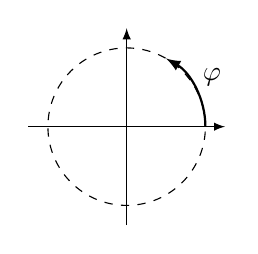
\begin{tikzpicture}
	\draw[-latex] (-1.25,0) -- (1.25,0);
	\draw[-latex] (0,-1.25) -- (0,1.25);
	\draw[dashed] (0,0) circle (1);
	\draw[thick,-latex] (1,0) arc (0:60:1);
	\node at (30:1.25) {$ \varphi $};
\end{tikzpicture}
		\end{minipage}
		\begin{minipage}{0.55\textwidth}
			\centering
			$ \begin{aligned}
				e_1 &\mapsto \begin{pmatrix} \cos \varphi \\ \sin \varphi \end{pmatrix} 
				\\ 
				e_2 &\mapsto \begin{pmatrix} -\sin \varphi \\ \cos \varphi \end{pmatrix} \\
				A &= \begin{pmatrix}
					\cos \varphi & -\sin \varphi \\
					\sin \varphi & \cos \varphi
				\end{pmatrix}
			\end{aligned} $
		\end{minipage}
	\end{figure}
	\noindent $ A^2 $ dreht einen Vektor um $ 2\varphi $. Demnach ist $ A^2 = \begin{pmatrix}
		\cos 2\varphi & -\sin 2\varphi \\
		\sin 2\varphi & \cos 2\varphi
	\end{pmatrix} $. Außerdem gilt:
	\begin{align*}
		p_A &= \det \begin{pmatrix}
			t - \cos \varphi & \sin \varphi \\
			-\sin \varphi & t - \cos \varphi
		\end{pmatrix} \\
		&= t^2 - 2t \cos \varphi + \cos^2 \varphi + \sin^2 \varphi \\
		&= t^2 - 2t \cos \varphi + 1
	\end{align*}
	Nach Cayley-Hamilton ist $ A^2 - 2 \cos \varphi \cdot A + I = 0 $, d.h.
	\begin{equation*}
		\begin{pmatrix}
			\cos 2\varphi & -\sin 2\varphi \\
			\sin 2\varphi & \cos 2\varphi
		\end{pmatrix} = 2 \cos \varphi \begin{pmatrix}
			\cos \varphi & -\sin \varphi \\
			\sin \varphi & \cos \varphi
		\end{pmatrix} - \begin{pmatrix}
			1 & 0 \\
			0 & 1
		\end{pmatrix}
	\end{equation*}
	Demzufolge ist 
	\[
		 \cos(2\varphi) = 2 \cos^2 \varphi - 1 
	\]
		und 
	\[ 
		\sin(2\varphi) = 2\sin\varphi\cos\varphi . 
	\]
	Das sind die bekannten Formeln für den Kosinus und Sinus des doppelten Winkels. Es kann sein, dass Sie diese Formeln bereits in der Schule hatten (in Mathematik oder Physik). Diese Formeln haben wir aus dem Satz von Cayley-Hamilton hergeleitet. Es gibt natürlich auch andere, direktere Möglichkeiten, die beiden Formeln herzuleiten. Uns geht in diesem Beispiel darum, das neue Wissen, das wir gerade erwerben mit dem alten Wissen zu verbinden (je mehr Verbindungen sehen wir, desto besser verstehen wir den Stoff). 
	
	Können wir auch Formeln für den Kosinus und Sinus des dreifachen Winkel herleiten? Der dreifache Winkeln hängt mit $A^3$ zusammen. Wir müssen also herausfinden, wie $A^3$ von $A$ abhängt. Wir wissen bereits, dass $A^2 =  2 \cos \varphi \, A - I$ gilt. Daher ist $A^3= A \cdot A^2 = A( 2 \cos \varphi A - I ) =   2 \cos \varphi A^2 - A $. Und dann können wir für $A^2$ den Ausdruck $2 \cos \varphi \, A - I $ noch einmal einsetzen. Das ergibt: 
	\[
		A^3 = 2 \cos \varphi (2 \cos \varphi A - I )= (4 \cos^2 \varphi -1) A - 2 \cos \varphi  I. 
	\]
	Wenn man nun die letzte Formel Komponentenweise ausschreibt sieh  man, wie man $\cos 3 \varphi$ und $\sin 3 \varphi$ mit Hilfe von $\cos \varphi$ und $\sin \varphi$ darstellen kann.
\end{bsp}

\begin{bem}
	Durch Cayley-Hamilton wird $ A^n $ ($ A \in \K^{n \times n} $) als Linearkombination von $ A^0, \ldots, A^{n-1} $ dargestellt. Man kann hierdurch die Potenzen $ A^k $ mit Hilfe der Multiplikation von Polynomen ausrechnen (vgl. Beispiel oben). Cayley-Hamilton hilft uns also im Ring $\K[A]$ zu rechnen. 
\end{bem}

\begin{bem}
	Sei $ A \in \K^{n \times n} $. Als Vektorraum über $ \K $ hat $ \K[A] $ die Dimension höchstens $ n $. (Übungsaufgabe)
\end{bem}

\begin{bem}
	Wir können verschiedene interessante algebraische Strukturen als $\K[A]$ umsetzen. Die Algebra $\K[A]$ ist also oft eine konkrete Matrix-basierte `Umsetzung' einer abstrakten algebraischen Struktur. Natürlich hat man auch die Verbindung in die andere Richtung: denn jede quadratische Matrix $A$ wird mit  der Algebra $\K[A]$ in Verbindung gesetzt.  Somit wird $A$ ein Element der Algebraischen Struktur $\K[A]$. 
\end{bem}

Quadratische Matrizen sind konkrete Analoga der linearen Abbildungen eines Vektorraums $V$. Wir können natürlich auch eine lineare Abbildung $F : V \to V$ in ein Polynom 
$ p = \sum_{i=1}^{d} c_it^i \in \K[t] $ einsetzen: wir definieren $p(F)$ als $ p(F) = \sum_{i=0}^{d} c_iF^i $. Auch in diesem Fall wird der Ring $ \K[F] := \set{q(F) : q \in \K[t]} $ eingeführt. Der Ring $\K[F]$ ist auch ein Untervektorraum von $\Lin(V)$. 

In der Sprache der linearen Abbildungen wird der Satz von Cayley-Hamilton folgendermaßen formuliert: 

\begin{thm}[Satz von Cayley-Hamilton für lineare Abbildungen]
	Sei $ V $ endlichdimensionaler Vektorraum und $ F : V \to V $ lineare Abbildung. Dann gilt:
	\begin{equation}
		p_F(F) = 0
	\end{equation}
\end{thm}
\begin{proof}
	Übungsaufgabe.
\end{proof}

\clearpage
\subsection{Diagonalisierbarkeit}

\subsubsection{Eine notwendige und eine hinreichende Bedingung}

Sei $ f \in \K[t] \setminus \set{0} $. $ f $ \emph{zerfällt in Linearfaktoren}, wenn $ f $ als $ f = c(t-\mu_1) \cdots (t-\mu_n) $ mit $ c \in \K \setminus \set{0} $ und $ \mu_1, \ldots, \mu_n \in \K $ darstellbar ist. Diese Eigenschaft ist von der Wahl von $ \K $ abhängig.

\begin{bspe}\
	\begin{enumerate}
		\item
			$ f = 3t^2-6t+3 \in \K[t] $ zerfällt für $ \K = \Q $ in Linearfaktoren, denn es ist \\
			$ f = 3(t-1)^2 $ ($ c=3 $ und $ \mu_1=\mu_2=1 $).
		\item
			$ f = t^2 - 2 \in \K[t] $ zerfällt für $ \K = \Q $ nicht in Linearfaktoren, aber bzgl. $ \K = \R $: \\
			$ f = (t-\sqrt{2})(t+\sqrt{2}) $.
	\end{enumerate}
\end{bspe}

\begin{thm}
	Sei $ V $ Vektorraum über $ \K $ mit $ \dim(V) = n \in \N $. Sei $ F \in \Lin(V) $. Dann gilt:
	\begin{enumerate}
		\item
			Ist $ F $ diagonalisierbar, so zerfällt $ p_F $ in Linearfaktoren.
		\item
			Ist $ p_F = (t-\mu_1) \cdots (t-\mu_n) $ mit paarweise verschiedenen $ \mu_1, \ldots, \mu_k \in \K $, d.h. $ p_F $ zerfällt in Linearfaktoren und hat $ n $ paarweise verschiedene Nullstellen, dann ist $ F $ diagonalisierbar.
	\end{enumerate}
\end{thm}
\begin{proof}\
	\begin{enumerate}
		\item
			Sei $ F $ diagonalisierbar, d.h. es existiert eine Basis $ \B $ von $ V $, für welche die Matrix $ F_\B $ diagonal ist.
			
			D.h. $ F_\B = \diag(\mu_1, \ldots, \mu_n) $ mit $ \mu_1, \ldots, \mu_n \in \K $ und es gilt $ p_F = p_{F_\B} = \det(tI - F_\B) = (t-\mu_1) \cdots (t-\mu_n) $. Also zerfällt $ p_F $ in Linearfaktoren.
		\item
			$ \mu_1, \ldots, \mu_n $ sind paarweise verschiedene Eigenwerte von $ F $. Aus Theorem \ref{sec:6_1_4} ergibt sich die Behauptung. \qedhere
	\end{enumerate}
\end{proof}

\subsubsection{Vielfachheit von Nullstellen und Zerlegbarkeit in Linearfaktoren}

\begin{propn}
	Sei $ f \in \K[t] \setminus \{ 0 \} $ und sei $ \lambda \in \K $ Nullstelle von $ f $. Dann existiert eine durch $ f $ und $ \lambda $ eindeutig bestimmte Zahl $ r \in \N $ und ein Polynom $ g \in \K[t] \setminus \{ 0 \} $ mit $ f = (t - \lambda)^r g $ und $ g(\lambda) \neq 0 $.
\end{propn}
\begin{proof}
	Aufgabe.
\end{proof}
\noindent Die Zahl $ r $ aus der vorigen Proposition nennt man die \emph{algebraische Vielfachheit} der Nullstelle $ \lambda $ von $ f $.
\begin{bem}
	$ r $ und $ g $ zu $ f $ lassen sich durch die iterative Verwendung der Polynomdivision bestimmen (vgl. Schule).
\end{bem}
\begin{propn}
	Sei $ f \in \K[t] \setminus \{ 0 \} $. Seien $ \lambda_1, \ldots, \lambda_k $ ($ k \in \N_0 $) die paarweise verschiedenen Nullstellen von $ f $. Dann kann $ f $ als das Produkt
	\begin{equation}
		f = (t - \lambda_1)^{r_1} \cdots (t - \lambda_k)^{r_k} g
		\label{eq:6_3_2}
	\end{equation}
	dargestellt werden, wobei $ r_1, \ldots, r_k \in \N $ mit $ g \in \K[t] \setminus \{ 0 \} $ keine Nullstellen in $ \K $ hat. Die vorige Darstellung ist bis auf die Nummerierung der Terme $ (t - \lambda_i)^{r_i} $ $ (i \in \is{1}{k}) $ eindeutig.
\end{propn}
\begin{proof}
	Aufgabe.
\end{proof}
\begin{bem}
	Die Darstellung \eqref{eq:6_3_2} lässt sich mit Hilfe der Polynomdivision bestimmen.
\end{bem}
\begin{bem}
	$ f $ zerfällt genau dann in Linearfaktoren, wenn in der Darstellung \eqref{eq:6_3_2} $ g $ eine Konstante ist, d.h. $ g \in \K \setminus \{ 0 \} $.
\end{bem}
\begin{bem}
	Zur Berechnung von \eqref{eq:6_3_2} muss die Menge $ \{ \lambda_1, \ldots, \lambda_k \} $ von $ f $ berechnet werden. Möglichkeiten dafür sind:
	\begin{enumerate}
		\item
			$ \K $ ist endlich $ \rightsquigarrow $ alle Elemente von $ \K $ durchprobieren (die direkte Methode).
		\item
			$ \K = \Q $. Man hat die folgende notwendige Bedingung. Sei $ f \in \Z[t] \setminus \{ 0 \} $ mit $ f = c_0 t^0 + \ldots + c_d t^d $ ($ c_0, \ldots, c_d \in \Z, c_d \neq 0, d \in \N $). Sei $ \lambda = \frac{a}{b} $ mit teilerfremden $ a,b \in \Z \setminus \{ 0 \} $ Nullstelle von $ f $, d.h. $ f(\lambda) = 0 $. Dann gilt:
			\begin{itemize}
				\item $ a $ teilt $ c_0 $
				\item $ b $ teilt $ c_d $
			\end{itemize}
			Dies sind wiederum endlich viele Möglichkeiten.
	\end{enumerate}
\end{bem}
%\clearpage
\begin{bspe}\
	\begin{enumerate}
		\item
			$ A = \begin{pmatrix}
				0 & 0 & 0 \\
				1 & 0 & 1 \\
				0 & 1 & 1
			\end{pmatrix} \in \K^{3 \times 3} $ mit $ \K = \Z/2\Z $. Dann ist
			
			$ p_A = \det\begin{pmatrix}
				t & 0 & 0 \\
				1 & t & 1 \\
				0 & 1 & t+1
			\end{pmatrix} = t^2(t+1) + t = t^3 + t^2 + t = t \underbrace{(t^2 + t + 1)}_{\mathclap{\text{\normalsize zerfällt nicht in Linearfaktoren}}} $.
			
			Es folgt: $ A $ ist nicht diagonalisierbar (bzgl. $ \K = \Z/2\Z $).
		\item
			$ A = \begin{pmatrix}
				0 & 0 & 0 \\
				1 & 0 & 1 \\
				0 & 1 & 1
			\end{pmatrix} \in \K^{3 \times 3} $ mit $ \K = \Q $. Dann ist
			
			$ p_A = \det\begin{pmatrix}
				t & 0 & 0 \\
				-1 & t & -1 \\
				0 & -1 & t-1
			\end{pmatrix} = t^2(t-1) - t = t^3 - t^2 - t = t\underbrace{(t^2 - t - 1)}_{\mathclap{\text{\normalsize hat keine Nullstellen in $ \Q $ }}} $.
			
			Es folgt: $ A $ ist bzgl. $ \K = \Q $ nicht diagonalisierbar.
		\item
			Sei $ A $ wie oben und $ \K = \R $. Man hat drei unterschiedliche Nullstellen: 0, $ \frac{1}{2} \pm \frac{\sqrt{5}}{2} $. D.h. $ p_A = t(t - \frac{1}{2} - \frac{\sqrt{5}}{2})(t - \frac{1}{2} + \frac{\sqrt{5}}{2}) $. Es folgt: $ A $ ist diagonalisierbar.
		\item
			Sei $ A = \begin{pmatrix}
				0 & -1 \\
				1 & 0
			\end{pmatrix} \in \K^{2 \times 2} $, $ \K=\R $.
			
			Es ist $ p_A = t^2 + 1 $. $ \lambda^2 + 1 \neq 0 \enspace \forall \lambda \in \R \Rightarrow $ bzgl. $ \K = \R $ zerfällt $ A $ nicht in Linearfaktoren.
		\item
			Sei $ A = \begin{pmatrix}
				0 & -1 \\
				1 & 0
			\end{pmatrix} \in \K^{2 \times 2} $, $ \K=\C $. Sei $ i $ die imaginäre Einheit, d.h. $ i^2 + 1 = 0 $.
			
			Es ist $ p_A = t^2 + 1 = (t-i)(t+i) $. $ \Rightarrow A $ ist diagonalisierbar.
		\item
			Sei $ A = O \in \K^{2 \times 2} $ und $ \K $ beliebig. Dann ist $ p_A = t^2 $. $ A $ ist diagonalisierbar (das Theorem aus 6.3.1 kann das aber nicht entscheiden).
		\item
			Sei $ A = \begin{pmatrix}
				0 & 1 \\
				0 & 0
			\end{pmatrix} \in \K^{2 \times 2} $ und $ \K $ beliebig. Dann ist $ p_A = t^2 $. $ A $ ist nicht diagonalisierbar (vgl. Kapitel 6...).
	\end{enumerate}
\end{bspe}

\subsubsection{Ungleichungen für die algebraische und die geometrische Vielfachheit}
\label{sec:6_3_3}

Sei $ V $ ein endlichdimensionaler Vektorraum über $ \K $ und sei $ F \in \Lin(V) $. Für die Diagonalisierbarkeit von $ F $ ist es notwendig, aber im allgemeinen Fall nicht hinreichend, dass $ p_F $ in Linearfaktoren zerfällt. Wir sind auf der Suche nach einer Bedingung an $ F $, die in Kombination mit der vorigen Bedingung an das charakteristische Polynom, die Diagonalisierbarkeit von $ F $ charakterisiert.

Sei $ \lambda $ Eigenwert von $ F $, d.h. $ p_F(\lambda) = 0 $. Die Vielfachheit von $ \lambda $ als Nullstelle von $ p_F $ nennt man die \emph{algebraische Vielfachheit} des Eigenwerts $ \lambda $ von $ F $.

Die Dimension von $ \Eig(F,\lambda) = \ker(F - \lambda \id) $ nennt man die \emph{geometrische Vielfachheit} des Eigenwerts $ \lambda $ von $ F $.

\begin{thm}
	Sei $ V $ $ n $-dimensionaler Vektorraum über $ \K $ mit $ n \in \N $ und sei $ F \in \Lin(V) $. Sei $ \lambda $ Eigenwert von $ F $. Sei $ k $ die geometrische Vielfachheit des Eigenwerts $ \lambda $ von $ F $ und $ l $ die algebraische Vielfachheit. Dann gilt: $ k \leq l $.
\end{thm}
\begin{proof}
	Sei $ b_1, \ldots, b_k $ eine Basis von $ \Eig(F,\lambda) = \{ v \in V : F(v) = \lambda v \} $. Wir erweitern $ b_1, \ldots, b_k $ zu einer Basis $ \B = (b_1, \ldots, b_n) $ von $ V $. Die Matrix $ F_\B $ hat die folgende Struktur:
	\begin{equation*}
		F_\B = \begin{pmatrix}
			\lambda I_k & C \\
			O & D
		\end{pmatrix}
	\end{equation*}
	mit $ C \in \K^{k \times (n-k)} $ und $ D \in \K^{(n-k) \times (n-k)} $. Es folgt: $ p_F = p_{F_\B} = \det(tI - F_\B) = \det((t - \lambda)I)_{k \times k}\det(tI - D)_{(n-k) \times (n-k)} = (t - \lambda)^k \det(tI - D) $. Es folgt, dass die algebraische Vielfachheit von $ l $ mindestens $ k $ ist.
\end{proof}

\subsubsection{Charakterisierung der Diagonalisierbarkeit}

\begin{thm}
	Sei $ V $ ein $ n $-dimensionaler Vektorraum über $ \K $ mit $ n \in \N $. Sei $ F \in \Lin(V) $. Dann sind die folgenden Bedingungen äquivalent:
	\begin{enumerate}
		\item
			$ F $ ist diagonalisierbar.
		\item
			Das charakteristische Polynom von $ F $ zerfällt in Linearfaktoren und für jeden Eigenwert $ \lambda $ von $ F $ sind die geometrische und die algebraische Vielfachheit von $ \lambda $ gleich.
		\item
			$ V $ ist direkte Summe der Eigenräume zu den Eigenwerten von $ F $.
	\end{enumerate}
\end{thm}
\begin{proof}\
	\begin{description}[font=\normalfont]
		\item[(i)$ \Rightarrow $(ii):]
			Sei $ F $ diagonalisierbar. Dann existiert eine Basis $ \B = (b_1, \ldots, b_n) $ und Werte $ \mu_1, \ldots, \mu_n \in \K $ mit $ F(b_i) = \mu_ib_i $ für alle $ i \in \is{1}{n} $. $ \Rightarrow $
			\begin{equation*}
				F_\B = \begin{pmatrix}
					\mu_1 && \\
					& \ddots & \\
					&& \mu_n
				\end{pmatrix}
				\quad\Rightarrow\quad
				p_F = p_{F_\B} = \det(tI - F_\B) = (t-\mu_1) \cdots (t-\mu_n),
			\end{equation*}
			also zerfällt $ p_F $ in Linearfaktoren. Sei $ \lambda $ beliebiger Eigenwert von $ F $ und sei $ r \in \K $ die algebraische Vielfachheit von $ \lambda $. Dann gilt $ \lambda = \mu_i $ für genau $ r $ unterschiedliche Indizes $ i \in \is{1}{n} $. O.B.d.A. sei $ \lambda = \mu_1 = \ldots = \mu_r $ und $ \lambda \neq \mu_i $ für $ i > r $. Somit sind $ b_1, \ldots, b_r $ linear unabhängige Eigenvektoren zu $ \lambda $, sodass die Ungleichung $ r = \dim(\lin(b_1, \ldots, b_r)) \leq \dim(\Eig(F,\lambda)) =: l $ erfüllt ist. Es folgt, dass die Gleichung $ r = l $ erfüllt ist, da die Ungleichung $ l \leq r $ in \ref*{sec:6_3_3} gezeigt wurde.
		\item[(ii)$ \Rightarrow $(iii):]
			Sei (ii) erfüllt. Seien $ \lambda_1, \ldots, \lambda_k $ ($ k \in \N $) die paarweise verschiedenen Nullstellen von $ p_F $. Wegen (ii) gilt $ p_F = (t-\lambda_1)^{r_1} \cdots (t-\lambda_k)^{r_k} $ mit $ r_1, \ldots, r_k \in \N $. Wegen (ii) gilt auch $ r_i = \dim(\Eig(F,\lambda_i)) $ für alle $ i \in \is{1}{n} $.
			
			Wir zeigen, dass die Summe der Räume $ \Eig(F,\lambda_i) $ mit $ i \in \is{1}{k} $ direkt ist. Seien $ v_i \in \Eig(F,\lambda_i) \enspace \forall i \in \is{1}{k} $ Vektoren mit $ v_1 + \ldots + v_k = 0 $. Da Eigenvektoren zu paarweise verschiedenen Eigenwerten linear unabhängig sind (Lemma \ref{sec:6_1_4}), folgt $ v_1 = \ldots = v_k = 0 $. Also ist die Summe der Räume $ \Eig(F,\lambda) $ mit $ i \in \is{1}{k} $ direkt. Für die Dimension dieser Summe gilt:
			\begin{align*}
				&\ \dim(\Eig(F,\lambda_1) \oplus \ldots \oplus \Eig(F,\lambda_k)) \\
				=&\ \dim(\Eig(F,\lambda_1)) + \ldots + \dim(\Eig(F,\lambda_k)) && \text{nach Theorem \ref{sec:3_6_4}} \\
				=&\ r_1 + \ldots + r_k && \text{wegen (ii)} \\
				=&\ n = \dim(V)
			\end{align*} %TODO: Formel aufhübschen!
			$ \Rightarrow \Eig(F,\lambda_1) \oplus \ldots \oplus \Eig(F,\lambda_k) = V $
		\item[(iii)$ \Rightarrow $(i):]
			Sei (iii) erfüllt und seien $ \lambda_1, \ldots, \lambda_k $ die Eigenwerte wie oben. Sei $ \B_i $ eine Basis von $ \Eig(F,\lambda_i) $ für $ i \in \is{1}{k} $. Wegen (iii) erhält man durch das Zusammenfügen der Systeme $ \B_1, \ldots, \B_k $ eine Basis $ \B $ von $ V $. Für diese Basis gilt
			\begin{equation*}
				F_\B = \begin{pmatrix}
					\lambda_1 I_{r_1} && \\
					& \ddots & \\
					&& \lambda_k I_{r_k}
				\end{pmatrix}
			\end{equation*}
			mit $ r_i = \dim(\Eig(F,\lambda_i)) \in \N \enspace \forall i \in \is{1}{k} $. Also ist $ F $ diagonalisierbar. \qedhere
	\end{description}
\end{proof}
\begin{bem}
	Das vorige Theorem zusammen mit Methoden zur Bestimmung von Nullstellen und Faktorisierung von Polynomen führt zu Rechenverfahren, welche die Diagonalisierbarkeit entscheiden können und gegebenenfalls eine Basis $ \B $ finden, für die $ F_\B $ diagonal ist:
	\begin{enumerate}[label=\arabic*.]
		\item Bestimme alle Eigenwerte der gegebenen Matrix und die jeweiligen algebraischen Vielfachheiten. 
		\item Berechne  zu jedem der Eigenwerte  eine Basis des Eigenraums (und somit auch die geometrische Vielfachheit). 
		\item Ist für einen der Eigenwerte die geometrische Vielfachheit ungleich der algebraischen Vielfachheit, dann ist die gegebene Matrix nicht diagonalisierbar. 
		\item Sonst ist die Matrix Diagonal in der Basis, die durch das Zusammenfügen der Basen der Eigenräume entsteht. 
	\end{enumerate} 
\end{bem}

